\documentclass[12pt,a4paper]{article}

% ─── Page Layout ───────────────────────────────────────────────────────────────
\usepackage[a4paper, margin=0.8in, headheight=14pt]{geometry}

% ─── Fonts (XeLaTeX) ───────────────────────────────────────────────────────────
\usepackage{fontspec}
\usepackage{unicode-math}
\setmainfont{TeX Gyre Pagella}
\setmonofont[Scale=0.88]{TeX Gyre Cursor}
\setmathfont{Latin Modern Math}

% ─── Packages ──────────────────────────────────────────────────────────────────
\usepackage{xcolor}
\usepackage{colortbl}
\usepackage{titlesec}
\usepackage{enumitem}
\usepackage{tabularx}
\usepackage{booktabs}
\usepackage{array}
\usepackage{amsmath}
\usepackage{tikz}
\usetikzlibrary{shapes.geometric, arrows.meta, positioning, calc, fit, decorations.pathreplacing}
\usepackage{tcolorbox}
\tcbuselibrary{skins, breakable}
\usepackage{hyperref}
\usepackage{fancyhdr}
\usepackage{graphicx}
\usepackage{microtype}
\hyphenpenalty=10000
\exhyphenpenalty=10000
\sloppy
\usepackage{caption}
\usepackage{setspace}
\usepackage{multirow}
\usepackage{tocloft}

% ─── Q&A helper ────────────────────────────────────────────────────────────────
\newcommand{\Q}[1]{\textbf{#1}\par\noindent\ignorespaces}

% ─── Colour Palette ────────────────────────────────────────────────────────────
\definecolor{myred}{RGB}{196,30,58}
\definecolor{mydark}{RGB}{30,30,50}
\definecolor{mygreen}{RGB}{14,120,80}
\definecolor{myteal}{RGB}{0,130,140}
\definecolor{myamber}{RGB}{180,100,0}
\definecolor{mypurple}{RGB}{100,30,160}
\definecolor{mygray}{RGB}{246,247,249}
\definecolor{mgframe}{RGB}{180,185,200}
\definecolor{watermark}{RGB}{145,150,170}
\definecolor{hdrred}{RGB}{250,232,235}
\definecolor{hdrgreen}{RGB}{220,244,233}
\definecolor{hdrteal}{RGB}{220,242,244}
\definecolor{hdramber}{RGB}{253,242,215}
\definecolor{hdrpurple}{RGB}{238,228,255}
\definecolor{hdrgray}{RGB}{238,240,245}
\definecolor{rowalt}{RGB}{250,251,253}

% ─── Section Formatting ────────────────────────────────────────────────────────
\titleformat{\section}
  {\large\bfseries\color{myred}}{\thesection.}{0.5em}{}
  [\vspace{1pt}{\color{myred}\rule{\linewidth}{0.8pt}}]
\titleformat{\subsection}
  {\normalsize\bfseries\color{myteal}}{\thesubsection}{0.5em}{}
\titlespacing*{\section}{0pt}{18pt}{7pt}
\titlespacing*{\subsection}{0pt}{11pt}{4pt}

% ─── Paragraph ─────────────────────────────────────────────────────────────────
\setlength{\parindent}{0pt}
\setlength{\parskip}{4pt}

% ─── TOC Styling ───────────────────────────────────────────────────────────────
\renewcommand{\cfttoctitlefont}{\large\bfseries\color{myred}}
\renewcommand{\cftaftertoctitle}{\par\noindent{\color{myred}\rule{\linewidth}{0.8pt}}}
\setlength{\cftbeforetoctitleskip}{0pt}
\setlength{\cftaftertoctitleskip}{6pt}
\renewcommand{\cftsecfont}{\normalsize\bfseries\color{mydark}}
\renewcommand{\cftsecpagefont}{\normalsize\bfseries\color{mydark}}
\renewcommand{\cftsecleader}{\cftdotfill{\cftdotsep}}
\setlength{\cftbeforesecskip}{7pt}
\renewcommand{\cftsubsecfont}{\small\color{mydark}}
\renewcommand{\cftsubsecpagefont}{\small\color{mydark}}
\setlength{\cftbeforesubsecskip}{3pt}
\setlength{\cftsubsecindent}{1.4em}

% ─── Table helpers ─────────────────────────────────────────────────────────────
\renewcommand{\arraystretch}{1.45}
\setlength{\tabcolsep}{6pt}
\arrayrulecolor{mydark}
\newcolumntype{B}[1]{>{\small\bfseries\raggedright\arraybackslash}m{#1}}
\newcolumntype{Y}{>{\small\raggedright\arraybackslash}X}
\renewcommand{\tabularxcolumn}[1]{m{#1}}

% ─── Header / Footer ───────────────────────────────────────────────────────────
\pagestyle{fancy}
\fancyhf{}
\fancyhead[L]{\small\color{myred}\textbf{OE-EC604C}\;\color{mydark}--- Object Oriented Programming}
\fancyhead[R]{\small\color{myteal}\textbf{Module 7 Notes}}
\fancyfoot[C]{\small\color{mydark}\thepage}
\fancyfoot[R]{\small\color{watermark}\textit{\copyright\ Biraj}}
\renewcommand{\headrulewidth}{0.5pt}
\renewcommand{\footrulewidth}{0.3pt}

% ─── Hyperref ──────────────────────────────────────────────────────────────────
\hypersetup{
  colorlinks=true, linkcolor=myteal, urlcolor=myteal,
  pdfauthor={Biraj Sarkar},
  pdftitle={OE-EC604C --- Module 7 Notes}
}

% ─── tcolorbox styles ──────────────────────────────────────────────────────────
\tcbset{
  tikzbox/.style={
    colback=mygray, colframe=mgframe, boxrule=0.6pt, arc=4pt,
    left=8pt, right=8pt, top=6pt, bottom=6pt,
    colbacktitle=mgframe, coltitle=mydark,
    fonttitle=\small\bfseries
  },
  defbox/.style={
    colback=hdrgreen, colframe=mygreen, boxrule=0.8pt, arc=4pt,
    left=9pt, right=9pt, top=6pt, bottom=6pt,
    colbacktitle=mygreen, coltitle=white,
    fonttitle=\small\bfseries
  },
  formulabox/.style={
    colback=hdrteal, colframe=myteal, boxrule=0.8pt, arc=4pt,
    left=9pt, right=9pt, top=7pt, bottom=7pt,
    colbacktitle=myteal, coltitle=white,
    fonttitle=\small\bfseries
  },
  examplebox/.style={
    colback=hdramber, colframe=myamber, boxrule=0.8pt, arc=4pt,
    left=9pt, right=9pt, top=6pt, bottom=6pt,
    colbacktitle=myamber, coltitle=white,
    fonttitle=\small\bfseries
  },
  masonbox/.style={
    colback=hdrpurple, colframe=mypurple, boxrule=0.8pt, arc=4pt,
    left=9pt, right=9pt, top=6pt, bottom=6pt,
    colbacktitle=mypurple, coltitle=white,
    fonttitle=\small\bfseries
  },
  exambox/.style={
    colback=hdrpurple, colframe=mypurple, boxrule=1pt, arc=5pt,
    left=10pt, right=10pt, top=8pt, bottom=8pt,
    colbacktitle=mypurple, coltitle=white,
    fonttitle=\bfseries,
    breakable, title after break={\textbf{Frequently Asked / Viva Questions (contd.)}}}
}

% XeLaTeX pdfcol fix: reset text color after every tcolorbox
\tcbset{after={\color{black}}}

% ─── TikZ styles ───────────────────────────────────────────────────────────────
\tikzset{
  block/.style={rectangle, draw=myteal, fill=hdrteal,
    text width=2.4cm, align=center, minimum height=0.95cm,
    font=\small, rounded corners=3pt, line width=0.7pt},
  redblock/.style={rectangle, draw=myred, fill=hdrred,
    text width=2.4cm, align=center, minimum height=0.95cm,
    font=\small, rounded corners=3pt, line width=0.7pt},
  netnode/.style={rectangle, draw=myteal, fill=hdrteal,
    text width=1.5cm, align=center, minimum height=0.8cm,
    font=\small, rounded corners=3pt, line width=0.7pt},
  sumjunc/.style={circle, draw=myamber, fill=hdramber,
    minimum size=0.62cm, font=\small, line width=0.8pt},
  snode/.style={circle, draw=mypurple, fill=hdrpurple,
    minimum size=0.55cm, font=\footnotesize, line width=0.7pt},
  arrow/.style={-Stealth, thick, color=mydark},
  redarrow/.style={-Stealth, thick, color=myred},
  line/.style={thick, color=mydark}
}

% ═══════════════════════════════════════════════════════════════════════════════
\begin{document}
% ═══════════════════════════════════════════════════════════════════════════════

\begin{center}
  {\LARGE\bfseries\color{myred} OE-EC604C --- Object Oriented Programming}\\[5pt]
  {\normalsize\color{mydark} Semester VI \quad$\bullet$\quad 3L:0T:0P \quad$\bullet$\quad 3 Credits}\\[3pt]
  {\normalsize\color{myteal}\textbf{Module 7 Exam Notes: Polymorphism}}\\[3pt]
  {\small\color{mydark} CGEC \;$|$\; B.Tech ECE (2023--27) \;$|$\; \textit{Biraj Sarkar}}
\end{center}
\vspace{2pt}
\noindent{\color{myred}\rule{\linewidth}{1.5pt}}
\vspace{2pt}

\hypersetup{linkcolor=mydark}
\tableofcontents
\hypersetup{linkcolor=myteal}
\newpage

% ===============================================================================
\section{Fundamentals of Polymorphism}
% ===============================================================================

Polymorphism ("many forms") allows a single interface to represent different underlying forms (behaviors). In C++, it is broadly classified into compile-time and run-time polymorphism.

\subsection{Pointers to Objects and Polymorphic Assignments}
Pointers can store the addresses of objects. In inheritance hierarchies, C++ supports upcasting:
\begin{tcolorbox}[defbox]
\textbf{Upcasting Rule:} A base class pointer can point to a derived class object without explicit typecasting. However, using this pointer, we can only access base class members, unless the functions are virtual.
\end{tcolorbox}
\begin{equation}
  \texttt{Base* ptr = new Derived(); // Polymorphic Assignment}
\end{equation}

\subsection{The \texorpdfstring{\texttt{this}}{this} Pointer}
The \texttt{this} pointer is an implicit parameter passed to all non-static member functions.
\textbf{Characteristics:}
\begin{itemize}[leftmargin=*, itemsep=2pt]
  \item It stores the address of the calling object.
  \item Used to resolve naming conflicts between member variables and parameters: \texttt{this->data = data;}.
  \item Used to return the calling object itself to enable \textbf{method chaining}: \texttt{return *this;}.
\end{itemize}

% ===============================================================================
\section{Compile-Time vs. Run-Time Polymorphism}
% ===============================================================================

The primary distinction lies in when the compiler resolves function invocations.

\subsection{Virtual Functions and Late Binding}
By prefixing a base class function declaration with the \texttt{virtual} keyword, we tell the compiler to resolve function calls at \textbf{run time} (late binding) based on the type of the object pointed to, rather than the type of the pointer.

\textbf{Mechanism of Late Binding (V-Table and V-Ptr):}
\begin{enumerate}[label=\textbf{\arabic*.}, leftmargin=*, itemsep=2.5pt]
  \item \textbf{V-Ptr (Virtual Pointer):} Every object of a class containing virtual functions is automatically allocated a hidden pointer field (\texttt{vptr}) pointing to its class's V-Table.
  \item \textbf{V-Table (Virtual Method Table):} A static table compiled for each class containing function addresses for all its virtual functions.
\end{enumerate}

\begin{tcolorbox}[tikzbox, title={Virtual Method Table (V-Table) Mapping Layout}]
\centering
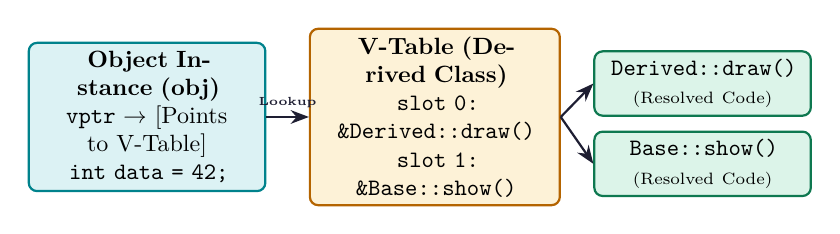
\begin{tikzpicture}[node distance=1.5cm, thick, scale=0.85, every node/.style={scale=0.85}]
  % Object Instance
  \node[rectangle, draw=myteal, fill=hdrteal, rounded corners=3pt, text width=3.3cm, align=center, minimum height=1.4cm] (obj) at (-3.5, 0) {
    \textbf{Object Instance (obj)}\\
    \texttt{vptr} $\rightarrow$ [Points to V-Table]\\
    \texttt{int data = 42;}
  };

  % V-Table
  \node[rectangle, draw=myamber, fill=hdramber, rounded corners=3pt, text width=3.5cm, align=center, minimum height=1.4cm] (vtable) at (0.8, 0) {
    \textbf{V-Table (Derived Class)}\\
    \texttt{slot 0:} \texttt{\&Derived::draw()}\\
    \texttt{slot 1:} \texttt{\&Base::show()}
  };

  % Code Segment
  \node[rectangle, draw=mygreen, fill=hdrgreen, rounded corners=3pt, text width=3.0cm, align=center, minimum height=0.7cm] (func0) at (4.8, 0.5) {
    \texttt{Derived::draw()}\\
    \scriptsize{(Resolved Code)}
  };
  \node[rectangle, draw=mygreen, fill=hdrgreen, rounded corners=3pt, text width=3.0cm, align=center, minimum height=0.7cm] (func1) at (4.8, -0.7) {
    \texttt{Base::show()}\\
    \scriptsize{(Resolved Code)}
  };

  % Arrows
  \draw[arrow] (obj.east) -- (vtable.west) node[midway, above, font=\tiny\bfseries] {Lookup};
  \draw[arrow] (vtable.east) -- (func0.west);
  \draw[arrow] (vtable.east) -- (func1.west);
\end{tikzpicture}
\end{tcolorbox}

\begin{tcolorbox}[examplebox, title={Code Example: Runtime polymorphism using base pointer arrays}]
\begin{spacing}{1.0}
\begin{verbatim}
#include <iostream>
class Shape {
public:
    virtual void draw() { // Virtual function
        std::cout << "Drawing generic shape" << std::endl;
    }
    virtual ~Shape() {} // Virtual destructor
};

class Circle : public Shape {
public:
    void draw() override { // Overridden function
        std::cout << "Drawing Circle" << std::endl;
    }
};

class Box : public Shape {
public:
    void draw() override {
        std::cout << "Drawing Box" << std::endl;
    }
};

int main() {
    Shape* shapes[2];
    shapes[0] = new Circle();
    shapes[1] = new Box();
    
    for(int i = 0; i < 2; i++) {
        shapes[i]->draw(); // Late binding: calls appropriate draw()
        delete shapes[i];
    }
    return 0;
}
\end{verbatim}
\end{spacing}
\end{tcolorbox}

% ===============================================================================
\section{Pure Virtual Functions and Abstract Classes}
% ===============================================================================

Sometimes, a base class is so generic that it cannot provide any logical default implementation for its virtual functions.

\subsection{Pure Virtual Functions}
\begin{tcolorbox}[defbox]
\textbf{Pure Virtual Function:} A virtual function declared in a base class with no implementation, represented by assigning \texttt{= 0} at its declaration.
\end{tcolorbox}
\begin{equation}
  \text{Declaration: } \quad \texttt{virtual}\;\text{Return\_Type}\;\text{FuncName}(\text{Args}) = 0;
\end{equation}

\subsection{Abstract Classes}
A class containing at least one pure virtual function is an \textbf{Abstract Class}.
\textbf{Key Characteristics:}
\begin{itemize}[leftmargin=*, itemsep=2.5pt]
  \item Instantiation: Abstract classes cannot be used to instantiate objects. E.g., \texttt{Employee emp;} is a compile error.
  \item Subclassing: Derived classes must override \textbf{all} inherited pure virtual functions to become concrete classes. Failure to do so makes the derived class abstract as well.
\end{itemize}

\begin{tcolorbox}[examplebox, title={Code Example: Abstract Employee base class}]
\begin{spacing}{1.0}
\begin{verbatim}
#include <iostream>
#include <string>
class Employee {
protected:
    std::string name;
public:
    Employee(std::string n) : name(n) {}
    virtual double calculateSalary() = 0; // Pure virtual function
    virtual void display() {
        std::cout << "Employee: " << name << std::endl;
    }
    virtual ~Employee() {}
};

class FullTimeEmployee : public Employee {
private:
    double monthlySalary;
public:
    FullTimeEmployee(std::string n, double s) : Employee(n), monthlySalary(s) {}
    double calculateSalary() override { return monthlySalary; }
};
\end{verbatim}
\end{spacing}
\end{tcolorbox}

% ===============================================================================
\section{Virtual Destructors \& Memory Leaks}
% ===============================================================================

When destroying dynamically allocated derived class objects through base class pointers, memory leaks will occur unless the base class destructor is virtual.

\subsection{Destructor Call Failures}
If the base class destructor is \textbf{non-virtual}, the compiler binds the destructor call to the base pointer type at compile time.
As a result, only the base class destructor executes. The derived class destructor never runs, leaving any heap allocations or handles inside the derived class unreleased.

\begin{tcolorbox}[examplebox, title={Code Example: Memory leak prevention via Virtual Destructors}]
\begin{spacing}{1.0}
\begin{verbatim}
#include <iostream>
class Base {
public:
    Base() { std::cout << "Base Constructor" << std::endl; }
    // Declaring destructor virtual guarantees derived deallocation
    virtual ~Base() { std::cout << "Base Destructor" << std::endl; }
};

class Derived : public Base {
private:
    int* data;
public:
    Derived() {
        std::cout << "Derived Constructor" << std::endl;
        data = new int[100]; // Heap allocation
    }
    ~Derived() {
        std::cout << "Derived Destructor (Releasing Heap)" << std::endl;
        delete[] data; // Releases resource safely
    }
};

int main() {
    Base* ptr = new Derived();
    delete ptr; // Triggers Derived destructor then Base destructor
    return 0;
}
\end{verbatim}
\end{spacing}
\end{tcolorbox}

% ===============================================================================
% MANDATORY QUICK REVISION PAGE
% ===============================================================================
\newpage
\begin{center}
  {\large\bfseries\color{myred} Quick Revision --- Module VII}\\[3pt]
  {\small\color{mydark} Polymorphism $|$ OE-EC604C}
\end{center}
\noindent{\color{myred}\rule{\linewidth}{1.2pt}}
\vspace{4pt}

\begin{tcolorbox}[formulabox, title={\textbf{Key Polymorphic Syntax}}]
\renewcommand{\arraystretch}{1.3}
\begin{tabularx}{\linewidth}{B{3.8cm} X}
Virtual Declaration      & \texttt{virtual void print(); // Inside base class declaration} \\[4pt]
Override Qualifier       & \texttt{void print() override; // Inside derived class (C++11)} \\[4pt]
Pure Virtual Function    & \texttt{virtual void process() = 0; // Defines abstract interface} \\[4pt]
Virtual Destructor       & \texttt{virtual \textasciitilde Base() \{ /* virtual base destructor */ \}}
\end{tabularx}
\end{tcolorbox}

\begin{tcolorbox}[defbox, title={\textbf{One-Line Definitions}}]
\begin{itemize}[leftmargin=*, itemsep=2.5pt, topsep=0pt]
  \item \textbf{Polymorphism:} The ability of different classes to respond uniquely to identical message calls.
  \item \textbf{Virtual Function:} A class member function overridden in derived classes to ensure late binding execution.
  \item \textbf{Late Binding:} Resolving function calls at run time based on the active object's type.
  \item \textbf{V-Table:} A compiler-generated static lookup table storing virtual function addresses for a class.
  \item \textbf{V-Ptr:} An object instance pointer referencing the V-Table allocated during object instantiation.
  \item \textbf{Pure Virtual Function:} An abstract base method initialized to \texttt{= 0} that derived classes must override.
  \item \textbf{Abstract Class:} A class containing pure virtual methods that cannot be instantiated.
  \item \textbf{Virtual Destructor:} A base class destructor configured to trigger proper intermediate subclass destructor sequences.
  \item \textbf{This Pointer:} An implicit member pointer storing the memory address of the calling object.
\end{itemize}
\end{tcolorbox}

\begin{tcolorbox}[exambox, title={\textbf{Frequently Asked / Viva Questions}}]
\begin{enumerate}[topsep=0pt, label=\textbf{Q\arabic*.}, itemsep=5pt]
  \item \Q{What is the difference between early binding and late binding?}
    Early binding (compile time) resolves function addresses using pointer types. Late binding (run time) resolves addresses using the pointed-to object type via the V-Table lookup.
  \item \Q{Can we declare a virtual function inside a structure (\texttt{struct})?}
    Yes. Structures in C++ are identical to classes but use public access by default. They support the \texttt{virtual} keyword and inheritance.
  \item \Q{What is the size impact of adding virtual functions to a class?}
    It adds the size of a single pointer (\texttt{vptr}) to every object instance (typically 4 bytes on 32-bit and 8 bytes on 64-bit systems), regardless of how many virtual functions are defined.
  \item \Q{Can a class have virtual static member functions?}
    No. Static member functions are class-wide and do not bind to object instances. Since they lack a \texttt{this} pointer and \texttt{vptr} links, they cannot be virtual.
  \item \Q{Can we override private virtual functions in C++?}
    Yes. The derived class can override private base virtual functions. Access levels only restrict calling permissions, not inheritance resolution.
  \item \Q{What is the difference between overloading and overriding?}
    Overloading occurs within the same class scope (same name, different arguments). Overriding occurs between base and derived classes (same name, identical arguments, uses \texttt{virtual}).
  \item \Q{Can an abstract class have constructors?}
    Yes. An abstract class cannot be instantiated directly, but its constructors run during derived class constructor sequences to initialize inherited data members.
  \item \Q{Why does a constructor declare base classes virtual during multiple derivations?}
    To bypass duplicate grandparent member allocations in hybrid structures (solving the Diamond Problem).
  \item \Q{What happens if we forget to declare base destructors virtual?}
    Deleting derived class instances through base class pointers only calls the base destructor, leaking derived heap resources.
  \item \Q{What is a pure abstract class or interface?}
    A class that contains \textit{only} pure virtual functions and no data members. It acts purely as a behavior contract.
  \item \Q{Can we call a virtual function from a constructor or destructor?}
    Yes, but early binding is used. It calls the local class's implementation, not the derived class's version, because the derived object is not yet fully constructed or is already destroyed.
  \item \Q{What is the purpose of the \texttt{override} keyword in C++11?}
    It instructs the compiler to verify that the function matches a virtual base class signature, preventing signature mismatch errors.
\end{enumerate}
\end{tcolorbox}

\begin{tcolorbox}[tikzbox, title={Comparison: Compile-Time vs. Run-Time Polymorphism}]
\renewcommand{\arraystretch}{1.45}
\par\noindent
\begin{tabularx}{\linewidth}{|B{3.2cm}|Y|Y|}
\hline
\textbf{Feature} & \textbf{\color{myteal}Compile-Time Polymorphism} & \textbf{\color{myamber}Run-Time Polymorphism} \\
\hline
\textbf{Binding Time} & resolved at compile time (Static Binding / Early Binding). & resolved at run time (Dynamic Binding / Late Binding). \\
\hline
\textbf{Mechanism} & Function Overloading and Operator Overloading. & Virtual Functions. \\
\hline
\textbf{Speed} & Fast execution (no run-time address lookup overhead). & Slightly slower (requires dereferencing the V-Ptr and V-Table lookup). \\
\hline
\textbf{Flexibility} & Fixed logic flow determined during compilation. & Highly flexible; handles new derived classes at runtime. \\
\hline
\textbf{Requirements} & Unique signatures (number/type of parameters). & Identical signatures; requires base pointer/reference interface. \\
\hline
\end{tabularx}
\end{tcolorbox}

\end{document}
